\documentclass{article}
\usepackage[active,tightpage]{preview}
\setlength{\PreviewBorder}{12pt}
\usepackage{tikz}
\usetikzlibrary{arrows.meta,external,decorations.pathmorphing,backgrounds,positioning,fit,calc}
\usepackage{amsmath}
\usepackage{amssymb}
\usepackage{amsfonts}

\PreviewEnvironment[{[]}]{tikzpicture}
\begin{document}

\tikzstyle{short_block} = [rectangle, text width = 4em, text centered, inner sep = 3pt, minimum height = 1.0em]

\tikzstyle{block} = [rectangle, text width = 5em, text centered, inner sep = 3pt, minimum height = 1.0em]

\tikzstyle{long_block} = [rectangle, text width = 12em, text centered, inner sep = 3pt, minimum height = 1.2em]

\tikzstyle{branchblock} = [rectangle, text width = 6em, text centered, inner sep = 3pt, minimum height = 1.8em]

\tikzstyle{cnn_block} = [rectangle, text width = 7em, text centered, inner sep = 3pt, minimum height = 1.2em]

\tikzstyle{mlp_block} = [rectangle, text width = 6em, text centered, inner sep = 3pt, minimum height = 1.2em]

\tikzstyle{phantom_block} = [rectangle, text width = 4em, text centered, inner sep = 3pt, minimum height = 1.3em]

\begin{tikzpicture}[node distance = 1cm, auto, arr/.style = {semithick, -Stealth}]

\node [block, fill = cyan!25] (input) at (0, 0) {Input};
% branch1
\node [branchblock, fill = red!25, below left = 0.5 and 1 of input] (b1) {ConvBranch1};
% branch2
\node [branchblock, fill = green!25, below = 0.5 of input] (b2) {ConvBranch2};
% branch3
\node [branchblock, fill = blue!25, below right = 0.5 and 1 of input] (b3) {ConvBranch3};
\node [phantom_block, fill = green!25, below = 0.53 of b2] (c2) {};
\node [phantom_block, fill = red!25, left = 0 of c2] (c1) {};
\node [phantom_block, fill = blue!25, right = 0 of c2] (c3) {};
\node [block, below = 0.5 of b2] (cat) {Concatenate};

\path[->] ([yshift = 5, xshift = -36]input.south) edge ([yshift = 2]b1.north);
\path[->] ([yshift = 5, xshift = 36]input.south) edge ([yshift = 2]b3.north);
\path[->] ([yshift = -2]input.south) edge ([yshift = 2]b2.north);
\path[->] ([yshift = -2, xshift = 10]b1.south) edge ([yshift = 2]c1.north);
\path[->] ([yshift = -2, xshift = -10]b3.south) edge ([yshift = 2]c3.north);
\path[->] ([yshift = -2]b2.south) edge ([yshift = 2]c2.north);

\node [long_block, fill = yellow!25, below = 0.5 of c2] (lstm) {$2\times$ BiLSTM(256) };
\node [long_block, fill = yellow!25, below = 0.5 of lstm] (attn) {Global Attention};
\node [long_block, fill = yellow!25, below = 0.5 of attn] (mlp) {MLP ($3\times$ Linear)};
\node [long_block, fill = yellow!25, below = 0.5 of mlp] (up) {Interpolate (scale=8)};
\node [block, fill = magenta!75, below = 0.5 of up] (out) {Output};

\path[->] ([yshift = -2]cat.south) edge ([yshift = 2]lstm.north);
\path[->] ([yshift = -2]lstm.south) edge ([yshift = 2]attn.north);
\path[->] ([yshift = -2]attn.south) edge ([yshift = 2]mlp.north);
\path[->] ([yshift = -2]mlp.south) edge ([yshift = 2]up.north);
\path[->] ([yshift = -2]up.south) edge ([yshift = 2]out.north);

\draw[dashed] ([xshift=-5,yshift=18]b1.west) rectangle ([xshift=5,yshift=-48]b3.east);
\node[long_block, above right = 0.8 and -1.8 of b3.east] (cnn) {\large\textbf{CNN Backbone}};
% \node [long_block, below left = 0.7 and -1.6 of b1] (cnn) {\large\textbf{CNN Backbone}};

\node [cnn_block, below right = 0.1 and 0.6 of b3] (bn) {\large\textbf{Branch N}};
\node [cnn_block, draw, below = 0.1 of bn] (conv1) {$1\times$ Conv-ReLU};
\node [cnn_block, draw, below = 0 of conv1] (bn1) {BatchNorm};
\node [cnn_block, draw, below = 0 of bn1] (mp1) {MaxPool(2)};
\node [cnn_block, draw, below = 0 of mp1] (conv2) {$2\times$ Conv-ReLU};
\node [cnn_block, draw, below = 0 of conv2] (bn2) {BatchNorm};
\node [cnn_block, draw, below = 0 of bn2] (mp2) {MaxPool(2)};
\node [cnn_block, draw, below = 0 of mp2] (dp) {Dropout(0.2)};
\node [cnn_block, draw, below = 0 of dp] (conv3) {$3\times$ Conv-ReLU};
\node [cnn_block, draw, below = 0 of conv3] (bn3) {BatchNorm};
\node [cnn_block, draw, below = 0 of bn3] (mp3) {MaxPool(2)};

\node [mlp_block, left = 0.4 of lstm] (mlp_) {\large\textbf{MLP}};
\node [mlp_block, draw, below = 0.1 of mlp_] (lin1) {Linear(256)};
\node [mlp_block, draw, below = 0 of lin1] (mi1) {Mish};
\node [mlp_block, draw, below = 0 of mi1] (dp1) {Dropout(0.2)};
\node [mlp_block, draw, below = 0 of dp1] (lin2) {Linear(64)};
\node [mlp_block, draw, below = 0 of lin2] (mi2) {Mish};
\node [mlp_block, draw, below = 0 of mi2] (dp2) {Dropout(0.2)};
\node [mlp_block, draw, below = 0 of dp2] (lin3) {Linear(1)};

\draw[black, rounded corners=20, thick] ([xshift=-25,yshift=45]b1.west) rectangle ([xshift=15,yshift=-20]mp3.east);

\node [below right = -2.9 and 1 of bn] (unet) {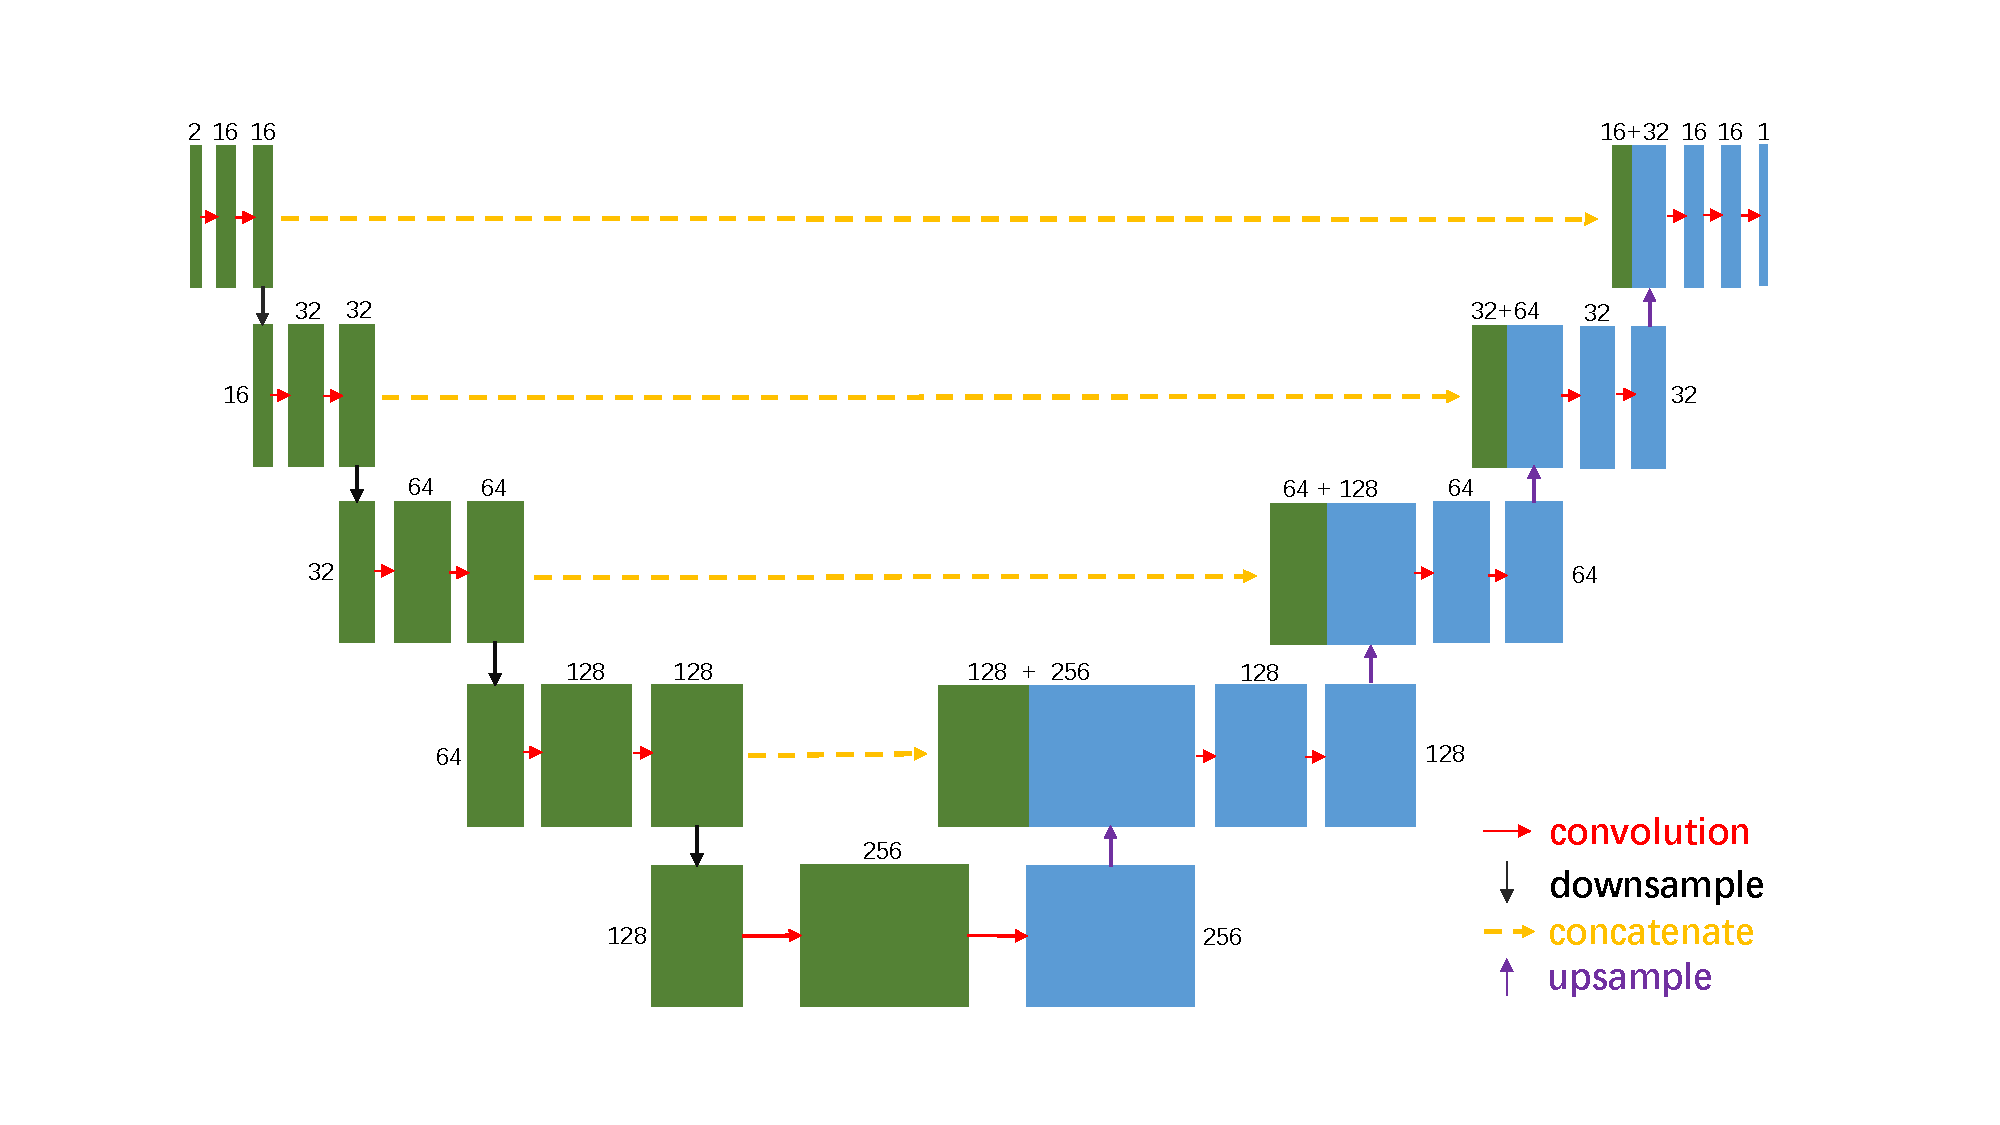
\includegraphics[width=1.1\textwidth]{images/unet.pdf}};
\draw[black, rounded corners=20, thick] ([xshift=25,yshift=100]unet.west) rectangle ([xshift=-25,yshift=-100]unet.east);

\node [above = 1.3 of b1] (seqtag) {\Large\textbf{SeqTag CRNN}};
\node [right = 20.3 of seqtag] (unet_text) {\Large\textbf{U-Net}};

\node [short_block, draw, below left = 1.2 and 3.55 of unet.south] (lstm_input) {RR};
\node [short_block, draw, right = 0.7 of lstm_input] (lstm) {BiLSTM};
\node [short_block, draw, right = 0.7 of lstm] (lstm_attn) {Attn};
\node [short_block, draw, right = 0.7 of lstm_attn] (lstm_mlp) {MLP};
\node [short_block, draw, right = 0.7 of lstm_mlp] (lstm_out) {Output};
\path[->] (lstm_input.east) edge (lstm.west);
\path[->] (lstm.east) edge (lstm_attn.west);
\path[->] (lstm_attn.east) edge (lstm_mlp.west);
\path[->] (lstm_mlp.east) edge (lstm_out.west);

\draw[black, rounded corners=5, thick] ([xshift=-7,yshift=13]lstm_input.west) rectangle ([xshift=7,yshift=-13]lstm_out.east);
\node [below left = 0.3 and -1.2 of lstm_out.south] (lstm_text) {\Large\textbf{RR LSTM}};

\node [below right = 2.7 and -11.2 of mp3.south] (example) {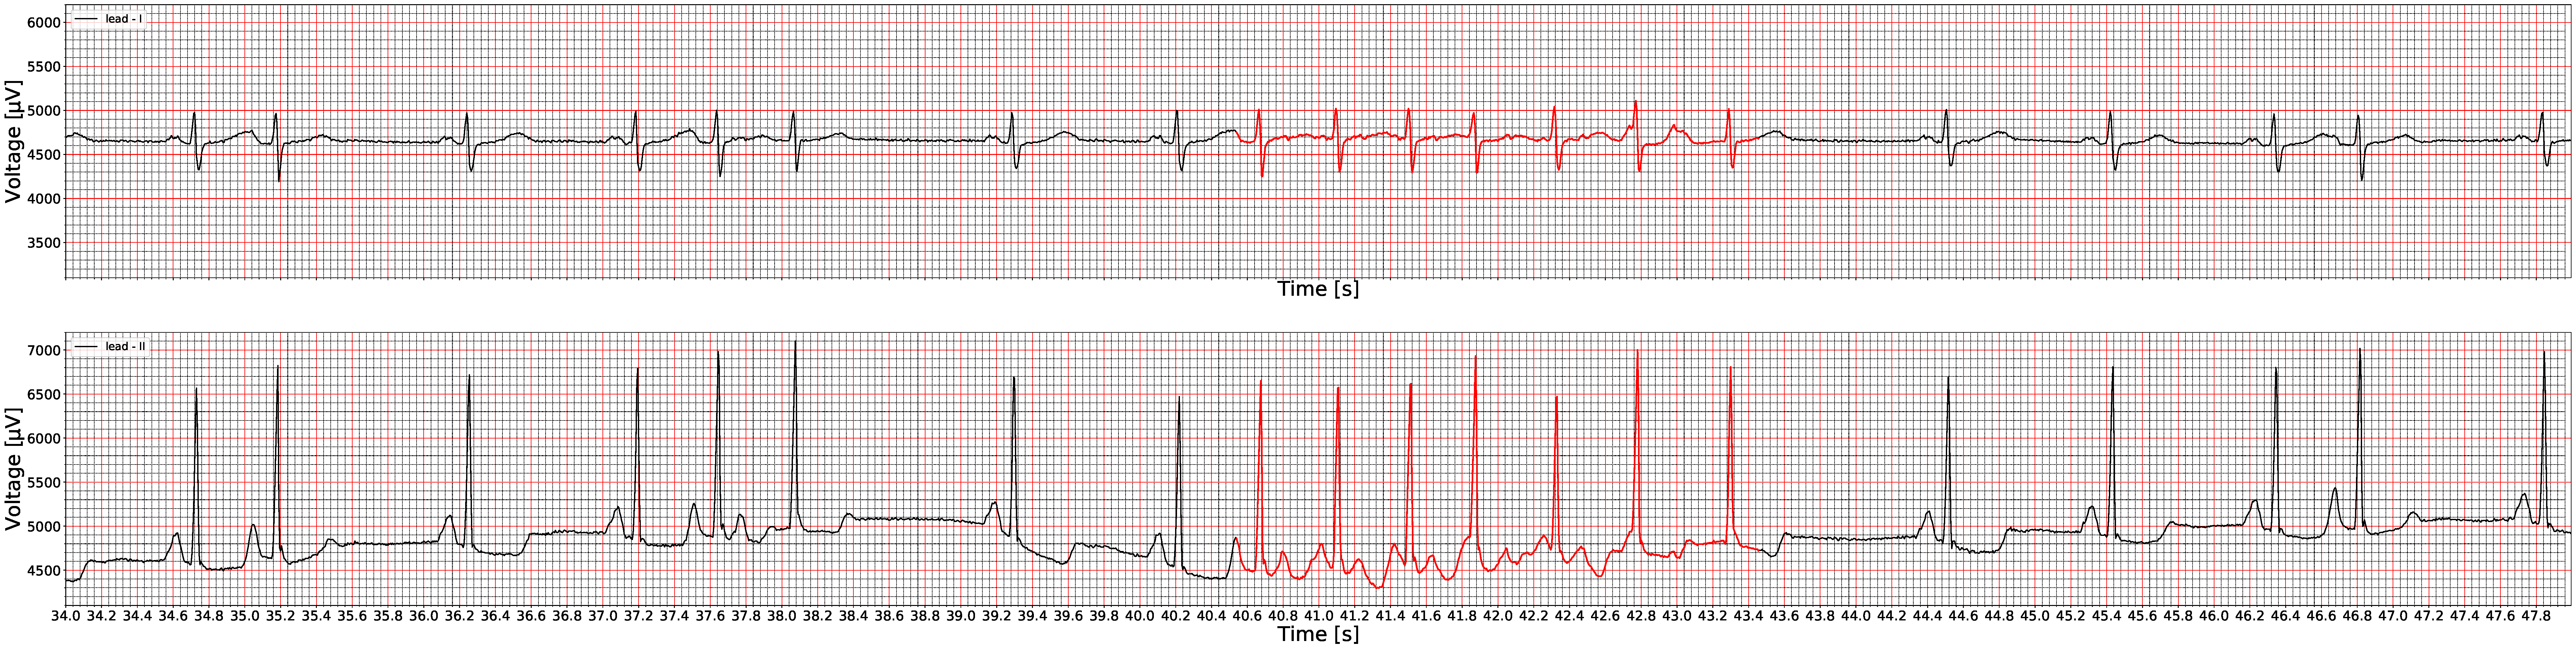
\includegraphics[width=2.13\textwidth]{images/cpsc2021_paf_event_example.pdf}};

\path[very thick, ->] ([yshift = -7]out.south) edge ([xshift=-50, yshift = 3]example.north);
\path[very thick, ->] ([xshift=-160, yshift = 5]unet.south) edge ([xshift=10, yshift = 3]example.north);
\path[very thick, ->] ([yshift = -15]lstm_attn.south) edge ([xshift=180, yshift = 3]example.north);

\node [above left = 0.1 and -0.1 of example.north] (afib) {\large\textbf{(AFIB}};
\path[very thick, dashed] (afib.south) edge ([yshift = -195]afib.south);
\node [above right = 0.1 and 5 of example.north] (n) {\large\textbf{(N}};
\path[very thick, dashed] (n.south) edge ([yshift = -195]n.south);

\node[left = 2.33 of afib] (paf) {\Large\textbf{Paroxysmal Atrial Fibrillation Event}};

\end{tikzpicture}

% \begin{tikzcd}
% \text{\framebox{Input}} \ar[r] & \text{\framebox{BiLSTM}} \ar[r] & \text{\framebox{Attn}} \ar[r] & \text{\framebox{MLP}} \ar[r] & \text{\framebox{Prediction}}
% \end{tikzcd}

\end{document}
